\documentclass[
	12pt,				% tamanho da fonte
	openany,			% capítulos começam em pág ímpar (insere página vazia caso preciso)
	oneside, 			% oneside - twoside
	a4paper,			% tamanho do papel.
	chapter=TITLE,		% títulos de capítulos convertidos em letras maiúsculas
	section=TITLE,		% títulos de seções convertidos em letras maiúsculas
	sumario=tradicional,	
	%subsection=TITLE,	% títulos de subseções convertidos em letras maiúsculas
	%subsubsection=TITLE,% títulos de subsubseções convertidos em letras maiúsculas
	english,			% idioma adicional para hifenização
	brazil,				% o último idioma é o principal do documento
	]{abntex2}

% ---------------------------------------------------------------------------
% Inclui os comandos do projeto
% ---------------------------------------------------------------------------
% -----------------------------------------------------------------------------
% Pacotes fundamentais
% -----------------------------------------------------------------------------
\usepackage{xcolor}
\newcommand\myworries[1]{\textcolor{red}{[#1]}}
\usepackage{lmodern}		% Usa a fonte Latin Modern (Serifada, tipo Times New Roman
%\usepackage{helvet}		% Usa a fonte Helvetica (Tipo Arial)	
%\renewcommand{\familydefault}{\sfdefault} tira o serifado
\usepackage[T1]{fontenc}		% Selecao de codigos de fonte.
\usepackage[utf8]{inputenc}		% Codificacao do documento (conversão automática dos acentos)
\usepackage{indentfirst}		% Indenta o primeiro parágrafo de cada seção.
\usepackage{color}				% Controle das cores
\usepackage{tikz}				% Inclusão de gráficos
\usepackage{graphicx}			% Inclusão de gráficos
\usepackage{microtype} 			% para melhorias de justificação
\usepackage{float}
% -----------------------------------------------------------------------------
% Pacotes adicionais, usados no anexo do modelo de folha de identificação
% -----------------------------------------------------------------------------
\usepackage{multicol}
\usepackage{multirow}
% -----------------------------------------------------------------------------
% Pacotes adicionais, usados apenas no âmbito do Modelo Canônico do abnteX2
% -----------------------------------------------------------------------------
\usepackage{lipsum}				% para geração de dummy text
% -----------------------------------------------------------------------------
% Pacotes de citações
% -----------------------------------------------------------------------------
\usepackage[brazilian,hyperpageref]{backref}	 % Paginas com as citações na bibliografia
\usepackage[alf,abnt-etal-list=3,abnt-etal-cite=3, abnt-emphasize=bf]{abntex2cite}	% Citações padrão ABNT
\usepackage{pdflscape}
\usepackage{footnote}
\usepackage{pdfpages}
\usepackage{caption}

% -----------------------------------------------------------------------------
% Pacotes adicionados por @leolleocomp
% ----------------------------------------------------------------------------- 
\usepackage{booktabs}
\usepackage{adjustbox}
\usepackage{subcaption}
\usepackage[labelfont=bf]{caption}
\usepackage{gensymb}
\usepackage{amsmath}
\usepackage{array}
\usepackage{float}
\usepackage{xcolor,colortbl}
\usepackage{longtable}
\usepackage{scalefnt}
\usepackage{listings}			% inserir codigo fonte


% -----------------------------------------------------------------------------
% Pacotes adicionados por @Gabrielr2508
% ----------------------------------------------------------------------------- 
\usepackage{hyperref}

\usepackage{tocloft}
% -- permite a adição de células especiais em tabelas
\newcommand{\specialcell}[2][c]{%
  \begin{tabular}[#1]{@{}c@{}}#2\end{tabular}}

\newcounter{equationset}
\newcommand{\equationset}[1]{% \equationset{<caption>}
  \refstepcounter{equationset}% Step counter
  \noindent\makebox[\linewidth]{Equação ~\theequationset: #1}
 }

%--------------------------------------------------------------------------------
% Adequação dos títulos dos capitulos, seções, subseções às normas da Univasf
% Added by @Gabrielr2508
%--------------------------------------------------------------------------------
\renewcommand{\ABNTEXchapterfont}{\fontseries{b}}
\renewcommand{\ABNTEXchapterfontsize}{\normalsize}

\renewcommand{\ABNTEXsectionfont}{\fontseries{m}}
\renewcommand{\ABNTEXsectionfontsize}{\normalsize}

\renewcommand{\ABNTEXsubsectionfont}{\fontseries{b}}
\renewcommand{\ABNTEXsubsectionfontsize}{\normalsize}

\renewcommand{\ABNTEXsubsubsectionfont}{\fontseries{m}}
\renewcommand{\ABNTEXsubsubsectionfontsize}{\normalsize}

%--------------------------------------------------------------------------------
% CONFIGURAÇÕES DE PACOTES
% Configurações do pacote backref
%--------------------------------------------------------------------------------
% Usado sem a opção hyperpageref de backref
\renewcommand{\backrefpagesname}{Citado na(s) página(s):~}
% Texto padrão antes do número das páginas
\renewcommand{\backref}{}
% Define os textos da citação
\renewcommand*{\backrefalt}[4]{
	\ifcase #1 %
		%Nenhuma citação no texto.%
	\or
		Citado na página #2.%
	\else
		Citado #1 vezes nas páginas #2.%
	\fi}%

%--------------------------------------------------------------------------------
% Configurações de aparência do PDF final
%--------------------------------------------------------------------------------
% alterando o aspecto da cor azul
\definecolor{blue}{RGB}{41,5,195}

% informações do PDF
\makeatletter
\hypersetup{
     	%pagebackref=true,
		pdftitle={\@title},
		pdfauthor={\@author},
    	pdfsubject={\imprimirpreambulo},
	    pdfcreator={LaTeX with abnTeX2},
		pdfkeywords={abnt}{latex}{abntex}{abntex2}{relatório técnico},
		colorlinks=true,			% false: boxed links; true: colored links
    	linkcolor=black,				% color of internal links
    	citecolor=black,				% color of links to bibliography
    	filecolor=black,			% color of file links
		urlcolor=black,
		bookmarksdepth=4
}
\makeatother
% ---

% ---
% Espaçamentos entre linhas e parágrafos
% ---

% O tamanho do parágrafo é dado por:
\setlength{\parindent}{1.3cm}

% Controle do espaçamento entre um parágrafo e outro:
\setlength{\parskip}{0.2cm}  % tente também \onelineskip

%--------------------------------------------------------------------------------
% compila o indice
%--------------------------------------------------------------------------------
\makeindex
% ---

%--------------------------------------------------------------------------------
% Comando para inserir imagens de forma simples
%--------------------------------------------------------------------------------
\newcommand{\imagem}[4]
{%			\imagem{x.x}{nomeimg}{titulo}{fonte}
	\begin{figure}[!htb]
		\caption{\label{img:#2}#3}
		\begin{center}
			\includegraphics[scale=#1]{img/#2}
		\end{center}
        \legend{\textbf{Fonte:} #4}
	\end{figure}
}%

%--------------------------------------------------------------------------------
% Creio que esses comandos sejam para desenhar algo, aguardando explicações de @leolleocomp
%--------------------------------------------------------------------------------
\newcommand{\xx} {$\bigotimes$}
\newcommand{\oo} {$\bigcirc$}

%--------------------------------------------------------------------------------
% Biblioteca para códigos-fonte
%--------------------------------------------------------------------------------
\usepackage[newfloat=true]{minted}

%--------------------------------------------------------------------------------
% Caixas batutas - by @leolleocomp
%--------------------------------------------------------------------------------
\usepackage[most]{tcolorbox}
\tcbuselibrary{breakable}

\tcbuselibrary{minted}
\tcbset{listing engine=minted}

\definecolor{bg}{rgb}{0.95,0.95,0.95}

\SetupFloatingEnvironment{listing}{name=Código, listname=Lista de códigos}

%--------------------------------------------------------------------------------
% configuração do contador dos códigos-fonte - by @leolleocomp
% assim como as figuras, começa em 1
\newcounter{sourcecode}
%--------------------------------------------------------------------------------
%--------------------------------------------------------------------------------
% @leolleocomp
% stackoverflow code
% peguei da resposta abaixo
% https://stackoverflow.com/questions/24086366/change-latex-minted-listings-numbering-to-include-current-section?answertab=votes#tab-top
%--------------------------------------------------------------------------------
\makeatletter
\renewcommand*{\thelisting}{\thesourcecode}
\makeatother

%--------------------------------------------------------------------------------
% Peçam explicações a @leolleo
% WHO DID THIS?
%--------------------------------------------------------------------------------
\newcommand{\Ididthis}{
%	\legend{\textbf{Fonte:} O autor (\the\year).}
\legend{\textbf{Fonte:} O autor}
}

\newcommand{\Otherguydidthis}[1]{
	\legend{\textbf{Fonte:} \citeonline{#1}.}
}

%--------------------------------------------------------------------------------
% Comando para inserir códigos - by @leolleocomp
%--------------------------------------------------------------------------------
\newcommand{\sourcecode}[4]{
\begin{listing}[H]
	\refstepcounter{sourcecode}
	\caption{#1}
	\label{cmd:#2}
	\inputminted[linenos, bgcolor=bg, tabsize=4,breaklines]{#3}{codes/#4}
	\Ididthis
\end{listing}
}



% ---------------------------------------------------------------------------
% IDENTIFICAÇÃO
% ---------------------------------------------------------------------------
\titulo{Experimento QSN-RI com $2^k$ fatores}
\autor{Daniele Silva Reis}
\local{JUAZEIRO - BA}
% \orientador{Prof. M. Sc. Ciclano Fulano de Tal}
%\coorientador{M. Sc. Osvaldo Campelo de Mello Vasconselos}
\instituicao{
UNIVERSIDADE FEDERAL DO VALE DO SÃO FRANCISCO
	\par
CURSO DE GRADUAÇÃO EM ENGENHARIA DE COMPUTAÇÃO}
% \tipotrabalho{Trabalho de Conclusão de Curso}
\preambulo{Relatório realizado para a disciplina de Avaliação e Desempenho de Sistemas, ministrada pelo Prof. Dr. Brauliro Gonçalves Leal, para obtenção de nota parcial.}


% -----------------------------------------------------------------------------
% CONFIGURACAO DO SUMARIO - by @Gabrielr2508
% Precisa estar aqui, por isso não foi para o commands.tex, não descobrimos o motivo, %caso saiba, por favor, faça um pull request! :D
% -----------------------------------------------------------------------------
% Secao primaria (Chapter) Caixa alta, Negrito, tamanho 12
\makeatletter
\renewcommand*{\l@chapter}[2]{%
  \l@chapapp{\uppercase{#1}}{#2}{\cftchaptername}}
\makeatother
% Secao secundaria (Section) Caixa baixa, Negrito, tamanho 12
\renewcommand{\cftsectionfont}{\uppercase} %ponha \rmfamily se quiser serifadas...

% Secao terciaria (Subsection) Caixa baixa, negrito, tamanho 12
\renewcommand{\cftsubsectionfont}{\bfseries}

% Secao quaternaria (Subsubsection) Caixa baixa, tamanho 12
\renewcommand{\cftsubsubsectionfont}{\normalfont}

% Seção quinaria (subsubsubsection) Caixa baixa, sem negrito, tamanho 12
\renewcommand{\cftparagraphfont}{\normalfont\itshape}

% -----------------------------------------------------------------------------
% Início do TCC 
% -----------------------------------------------------------------------------
\begin{document}

	\frenchspacing % Retira espaço extra obsoleto entre as frases.
	
	\pretextual
		%--------------------------------------------------------------------------------
% Constrói a capa com base na seção de identificação do main.tex
%--------------------------------------------------------------------------------
\begin{capa}
\center
	
\includegraphics[scale=0.6]{img/univasf.jpg}

	{\ABNTEXchapterfont\bfseries\large\imprimirinstituicao}

	\vspace*{5cm}
	{\ABNTEXchapterfont\bfseries\large\imprimirautor}

	\vfill
	{\ABNTEXchapterfont\bfseries\large\imprimirtitulo}
	\vfill
	\ABNTEXchapterfont\bfseries\large\imprimirlocal\\ \the\year

	\vspace*{1cm}

\end{capa}
%--------------------------------------------------------------------------------
% Constrói a folha de rosto com base na seção de identificação do main.tex
%--------------------------------------------------------------------------------
\begin{folhaderosto}
\center
		{\ABNTEXchapterfont\bfseries\large\imprimirautor}
		\vspace*{\fill}

		{\ABNTEXchapterfont\bfseries\large\imprimirtitulo}
		\vspace*{\fill}

		{\hspace{.45\textwidth}
		\begin{minipage}{.5\textwidth}
			\SingleSpacing
			\imprimirpreambulo \\ \\

			{\imprimirorientadorRotulo~\imprimirorientador\par}
			{\imprimircoorientadorRotulo~\imprimircoorientador\par}

		\end{minipage}%
		\vspace*{\fill}}%
		\vspace*{\fill}
			\ABNTEXchapterfont\bfseries\large\imprimirlocal\\ \the\year
		\vspace*{1cm}
\end{folhaderosto}

%--------------------------------------------------------------------------------
% Constrói a ficha catalográfia com base na seção de identificação do main.tex
% Está comentado porque no final das contas a biblioteca do seu campus que gera a 
% numeração, você pode adicionar os numeros aqui, ou anexar o pdf gerado por eles
% ao documento.
%--------------------------------------------------------------------------------
%\begin{fichacatalografica}
%	\vspace*{\fill}					% Posição vertical
%	\hrule							% Linha horizontal
%	\begin{center}					% Minipage Centralizado
%	\begin{minipage}[c]{12.5cm}		% Largura
%
%	\imprimirautor
%
%	\hspace{0.5cm} \imprimirtitulo  / \imprimirautor. --
%	\imprimirlocal, \the\year-
%
%	\hspace{0.5cm} xx p. : il. (algumas color.) ; 30 cm.\\
%
%	\hspace{0.5cm} \imprimirorientadorRotulo~\imprimirorientador\\
%
%	\hspace{0.5cm}
%	\parbox[t]{\textwidth}{\imprimirtipotrabalho~--~\imprimirinstituicao,
%	\the\year.}\\
%
%	\hspace{0.5cm}
%		1. Palavra-chave1.
%		2. Palavra-chave2.
%		I. Orientador.
%		II. Universidade xxx.
%		III. Faculdade de xxx.
%		IV. Título\\
%
%	\hspace{8.75cm} CDU 02:141:005.7\\
%
%	\end{minipage}
%	\end{center}
%	\hrule
%\end{fichacatalografica}

%--------------------------------------------------------------------------------
% Anexando a ficha catalogáfica e a folha de aprovação 
%--------------------------------------------------------------------------------
% 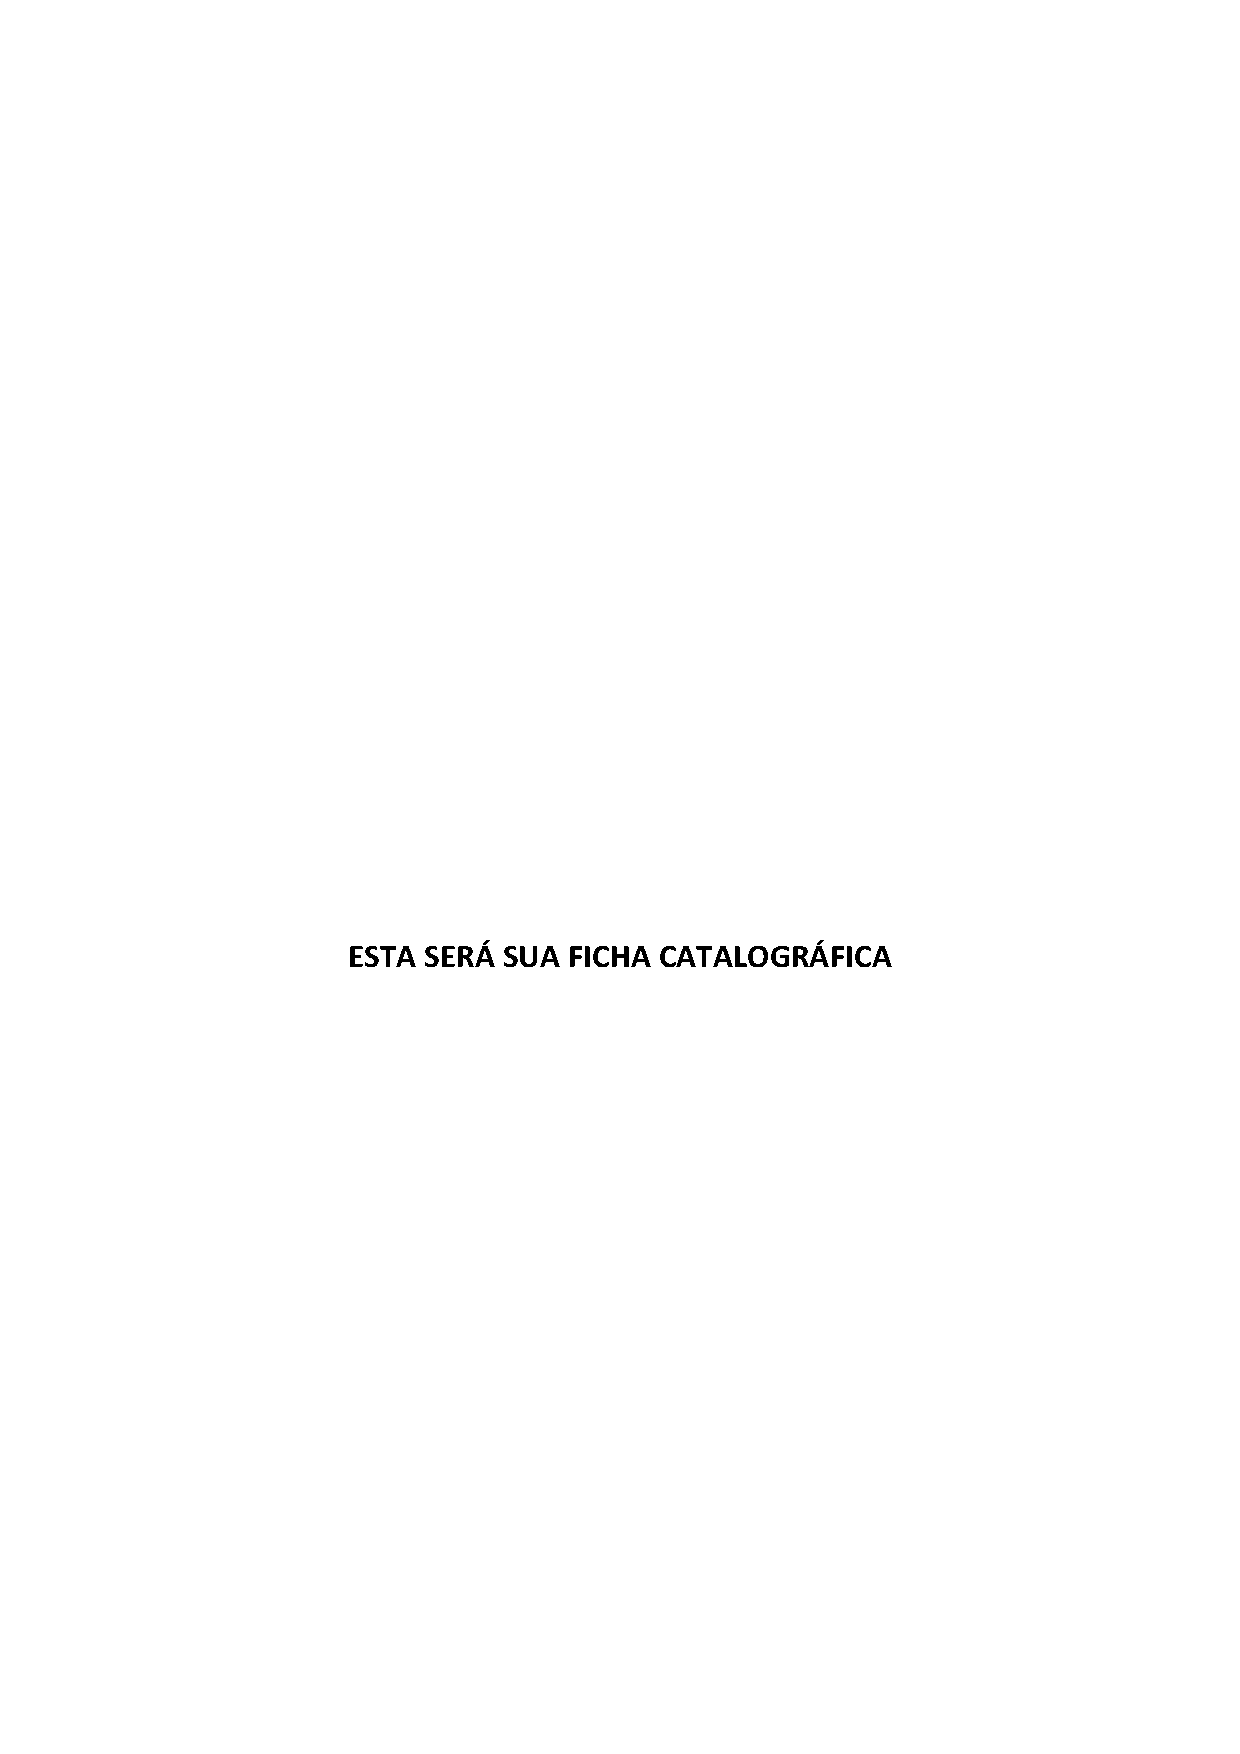
\includepdf[pages=-]{anexos/ficha.pdf}

% 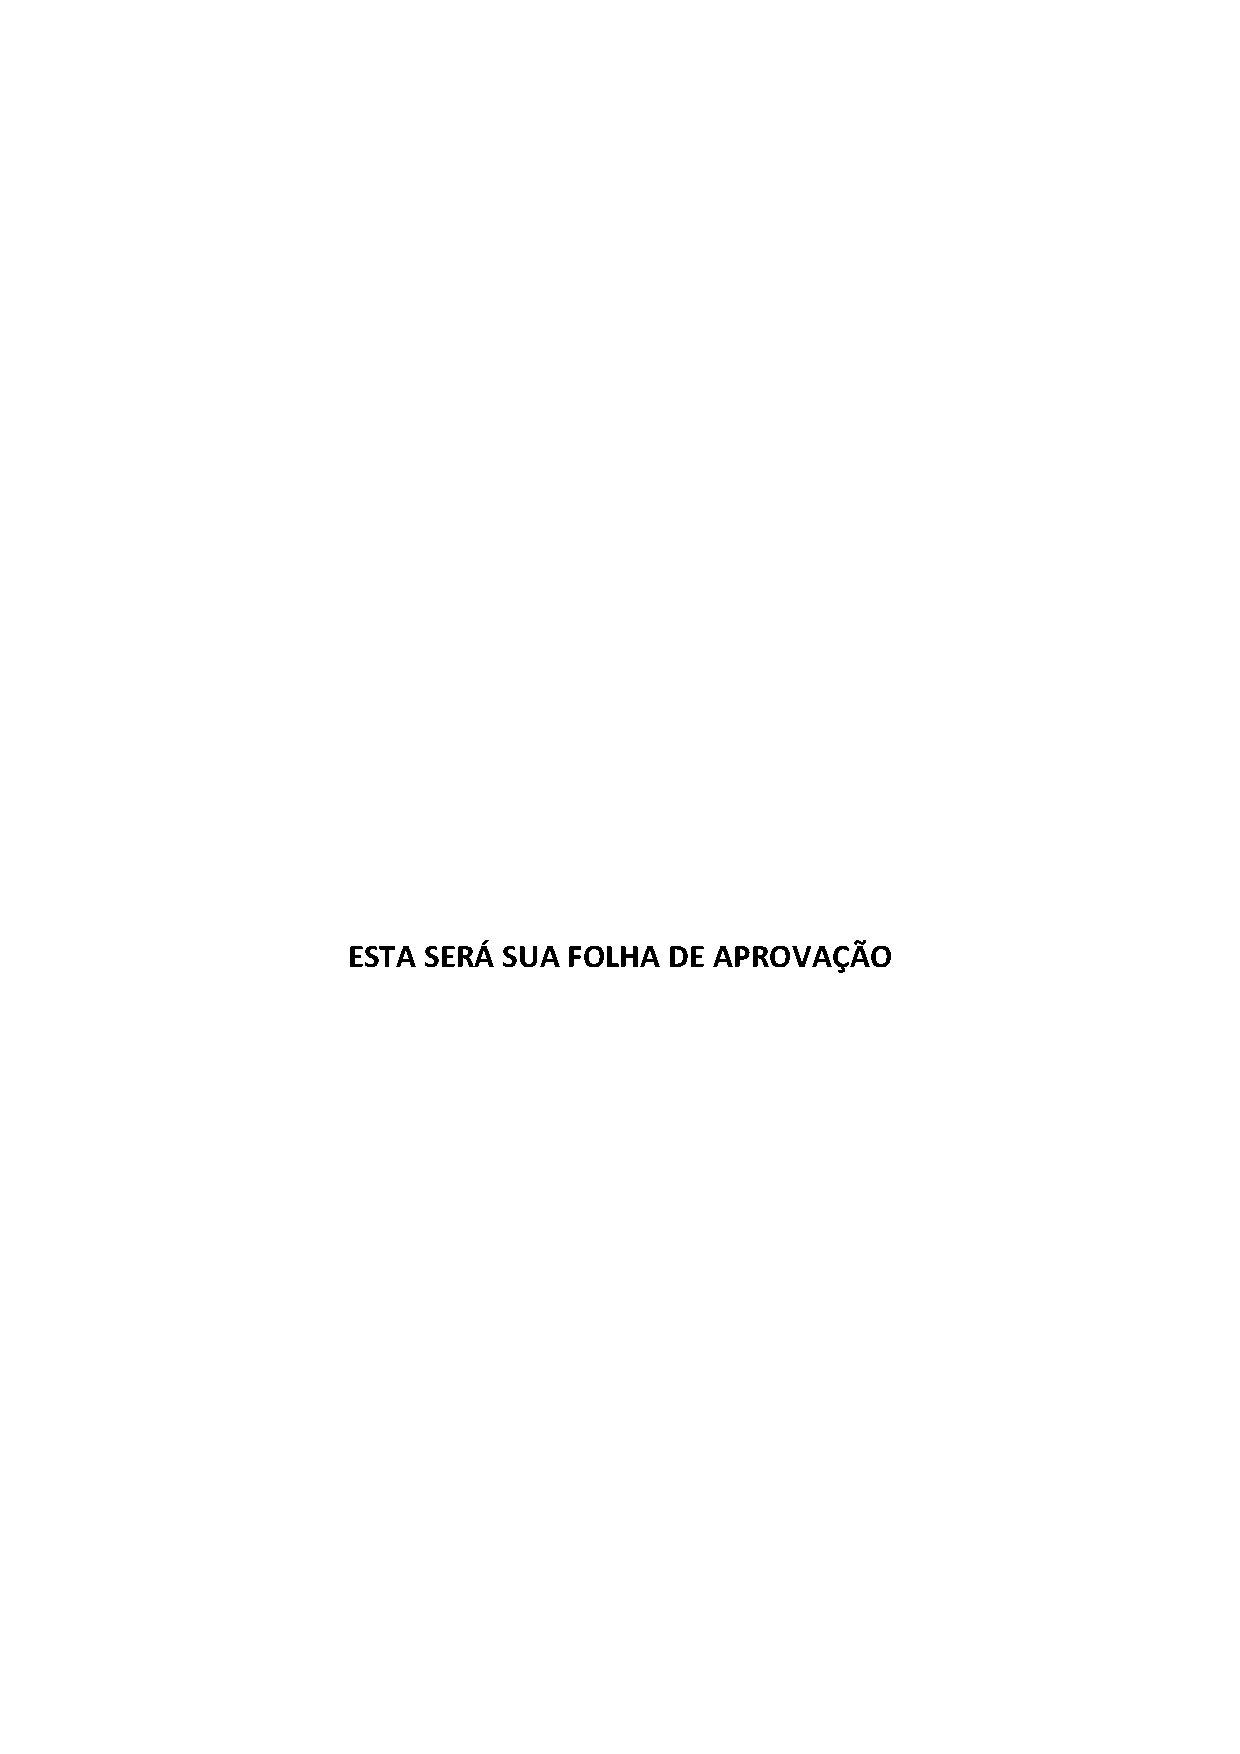
\includepdf[pages=-]{anexos/aprovacao.pdf}

\setlength{\ABNTEXsignwidth}{12cm}

%--------------------------------------------------------------------------------
% Está comentado pelo mesmo motivo da ficha catalográfica 
%--------------------------------------------------------------------------------
%\begin{folhadeaprovacao}
%	\begin{center}
%	    {\ABNTEXchapterfont\bfseries\large\imprimirinstituicao}
%	    \vspace*{\fill}
%
%	    {\ABNTEXchapterfont\bfseries\large FOLHA DE APROVAÇÃO}
%	    \vspace*{\fill}
%
%	    {\ABNTEXchapterfont\bfseries\large\imprimirautor}
%
%	    \vspace*{\fill}\vspace*{\fill}
%	    {\ABNTEXchapterfont\bfseries\large\imprimirtitulo}
%	    \vspace*{\fill}
%
%	    {\hspace{.45\textwidth}
%		\begin{minipage}{.5\textwidth}
%			\SingleSpacing
%			\ABNTEXchapterfont\imprimirpreambulo \\ \\
%
%			{\ABNTEXchapterfont\imprimirorientadorRotulo~\imprimirorientador\par}
%			{\ABNTEXchapterfont\imprimircoorientadorRotulo~\imprimircoorientador\par}
%
%		\end{minipage}%
%	    \vspace*{\fill}}
%	\end{center}
%
%	\vspace*{\fill}	
%	
%	\begin{center}
%			 \ABNTEXchapterfont\large Aprovado em: \_\_\_\_ de \_\_\_\_ de 2017
%	\end{center}

%	\vspace*{\fill}
	
%	\begin{center}
%			 \ABNTEXchapterfont\bfseries\large Banca Examinadora
%	\end{center}
%		
%   \ABNTEXchapterfont\assinatura{Fábio Nelson de Sousa Pereira, Mestre, Universidade Federal do Vale do São Francisco}
%	\ABNTEXchapterfont\assinatura{Jorge Luis Cavalcanti Ramos, Doutor, Universidade Federal do vale do São Francisco}
%  \ABNTEXchapterfont\assinatura{Ricardo Argenton Ramos, Doutor, Universidade Federal do Vale do São Francisco}
%	 \vspace*{\fill}

	 
%\end{folhadeaprovacao}

%--------------------------------------------------------------------------------
% Insere a epígrafe
%--------------------------------------------------------------------------------
% \newpage
% \vspace*{\fill}
% \begin{flushright}
% 		\textit{Lorem Ipsum...}
% \end{flushright}

% %--------------------------------------------------------------------------------
% % Seção de agradecimentos
% %--------------------------------------------------------------------------------
% \begin{agradecimentos}
	
% \lipsum[2-4]

% \end{agradecimentos}

% %--------------------------------------------------------------------------------
% % Insere a segunda epígrafe
% %--------------------------------------------------------------------------------
% \begin{epigrafe}
%     \vspace*{\fill}
% 	\begin{flushright}
% 		Se pude enxergar a tão grande distância, foi subindo nos ombros de gigantes.\\
% 		 \vspace{\baselineskip}
% 		\textbf{Isaac Newton}\\
% 		\textbf{Carta à Robert Hooke, 1676}
% 	\end{flushright}
% \end{epigrafe}



%--------------------------------------------------------------------------------
% Seção de resumos
%--------------------------------------------------------------------------------
% resumo em português
\setlength{\absparsep}{18pt} % ajusta o espaçamento dos parágrafos do resumo
\begin{resumo}

% Neste trabalho foram comparados os resultados da análise de desempenho de um sistema computacional através das técnicas QSN-RI e Análise do Valor Médio. O sistema utilizado é composto por 5 componentes, sendo estes um roteador, \textit{switch}, servidor de e-mail, computador de mesa e um \textit{notebook}, através do qual foi simulado o envio e recebimento de um e-mail na rede. O único parâmetro de entrada comum entre ambas as técnicas, além do tempo de serviço dos dispositivos, é o número de tarefas, que neste trabalho foi igual a 1000. A partir dos resultados obtidos, constatou-se uma subutilização do roteador, \textit{switch} e servidor. O computador e \textit{notebook} apresentaram as utilizações mais altas, com o \textit{notebook} alcançando valores iguais a 0,99. A partir da análise de gargalos, confirmou-se que este componente era o responsável pelo estrangulamento do sistema. Esta técnica forneceu, também, o número máximo de usuários sem que o sistema gargale, sendo igual a 73.

 \textbf{Palavras-chave}: Sistema Computacional. Avaliação de sistemas. Métricas de desempenho.

\end{resumo}

%---------------------------------------------------------------------------------
% resumo em inglês
% \begin{resumo}[Abstract]
% \begin{otherlanguage*}{english}

% \lipsum[3-4]
	
% 	\vspace{\onelineskip}

% 	\noindent
% 	\textbf{Key-words}: \textit{Palavra em inglês 1, Palavra em inglês 2, Palavra em inglês 3, Palavra em inglês 4, Palavra em inglês 4}.

% \end{otherlanguage*}
% \end{resumo}


%---------------------------------------------------------------------------------
% Insere lista de ilustrações
%---------------------------------------------------------------------------------
\begin{KeepFromToc} % Este comando evita que todas as seções dentro dele de apareçam no sumário
\pdfbookmark[0]{\listfigurename}{lof}
\listoffigures
%\addcontentsline{toc}{chapter}{Lista de Figuras}
\cleardoublepage


%---------------------------------------------------------------------------------
% Insere lista de tabelas
%---------------------------------------------------------------------------------
\pdfbookmark[0]{\listtablename}{lot}
\listoftables
\cleardoublepage

%---------------------------------------------------------------------------------
% Ajusta lista de código - alterar de figures para códigos - by @Gabrielr2508
%---------------------------------------------------------------------------------
% \makeatletter
% \let\l@listing\l@figure
% \def\newfloat@listoflisting@hook{\let\figurename\listingname}
% \makeatother

%---------------------------------------------------------------------------------
% Insere lista de códigos - by @leolleocomp
%---------------------------------------------------------------------------------
% \listoflistings

\end{KeepFromToc}

%---------------------------------------------------------------------------------
% Insere lista de abreviaturas e siglas
%---------------------------------------------------------------------------------
% \begin{siglas}
% 	\item[LI]       Lorem Ipsum
%     \item[LII]		Lorem Ipsum Ipsum
	    
% \end{siglas}

%---------------------------------------------------------------------------------
% Insere o sumario
%---------------------------------------------------------------------------------
\pdfbookmark[0]{\contentsname}{toc} 
\tableofcontents*
\cleardoublepage


	\textual
		\pagestyle{simple}
		%--------------------------------------------------------------------------------------
% Este arquivo contém a sua introdução, objetivos e organização do trabalho
%--------------------------------------------------------------------------------------
\chapter{Introdução}

As técnicas de avaliação de desempenhos de sistemas computacionais são úteis para que, através da estimativa do desempenho de um sistema similar ao que deseja-se desenvolver, possa-se determinar as configurações ideais dos componentes pertencentes ao sistema. A técnica QSN-RI fornece resultados objetivos quanto à utilização dos componentes, seu tempos de espera e de resposta e tamanho da fila. Ela recebe como parâmetros o tempo de serviço dos componentes, número de tarefas, o intervalo entre visitas, o número de repetições, a quantidade total de visita aos componentes e a ordem das visitas à eles.

Quando aliada à experimentos de $2^k$ fatores, é possível obter um diagnóstico completo quanto aos equipamentos que mais impactam no desempenho do sistema como um todo. Como este experimento é realizado para cada combinação de configuração dos componentes, é possível determinar os modelos mais adequados dos equipamentos.

Dessa forma, será conduzido um experimento com $k$ = 5 fatores, resultando em 32 combinações. A partir dos resultados obtidos, serão determinados os impactos de cada componente no sistema, assim como a configuração mais adequada para um melhor desempenho dele.

% \lipsum[5-10]


% \section{Objetivos gerais}

% \lipsum[1]

% \section{Objetivos específicos}

% \begin{itemize}
% 	\item blablablabla;
%     \item blablablabla;
%     \item blablablabla.
% \end{itemize}

% \section{Organização do trabalho}

% \lipsum[10-12]

		%--------------------------------------------------------------------------------------
% Este arquivo contém a sua metodologia
%--------------------------------------------------------------------------------------
\chapter{Metodologia} \label{ch:MM} %Uma label é como você referencia uma seção no texto com a tag \ref{}

O Sistema Computacional proposto conta com cinco componentes, dados por um \textit{switch}, roteador, servidor \textit{Web}, servidor de aplicação e servidor de banco de dados, como mostrado na Figura \ref{img:modelo}.

\begin{figure}[H]
    \centering
        \caption{\label{img:modelo} Sistema computacional escolhido.}
        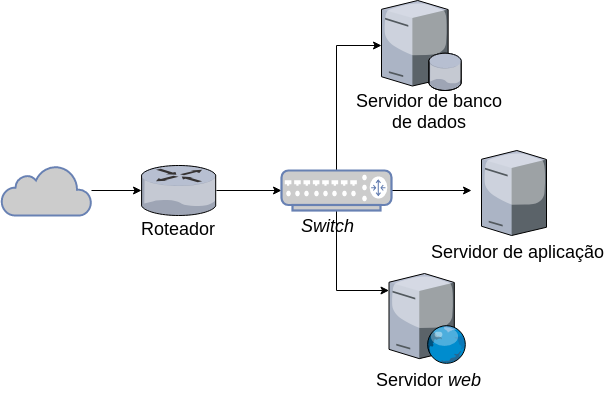
\includegraphics[scale=0.5]{img/modelo.png}
        \legend{\textbf{Fonte: } (Autor, 2019).}
    \end{figure}

Considerando 3000000 pacotes diários, o intervalo entre chegadas foi dado por:

\begin{equation*}
    iat = {\frac{3000000}{24*60*60}}^{-1} = 0,0288 s
\end{equation*}

Por outro lado, os tempos de serviço para cada nível de cada componente são mostrados na Tabela \ref{tbl:componentes}, considerando um pacote de tamanho 5,6 kB.

\begin{table}[!htb]
    \centering
    \caption{\label{tbl:componentes} Descrição dos componentes utilizados.}
        \begin{tabular}{ccm{2.2cm}m{1.9cm}m{2.9cm}m{2.5cm}m{1.6cm}}
            \hline
            \multicolumn{2}{c}{Nível/Fator} & Roteador (A) & \textit{Switch (B)} & Servidor de banco de dados (C) & Servidor de aplicação (D) & Servidor \textit{web} (E) \\ \hline
            \multirow{2}{*}{-1} & Modelo & Model 4451 & SF300-08P & Cassandra & Node.js 10.0.0 & Apache \\
            & $st$ ($10^{-5}$ s/tarefa) & $0,534$ & $0,333$ & $1146,8$ & $1,44$ & $71$ \\ \hline 
            \multirow{2}{*}{+1} & Modelo & Model 4461 & SF300-24P & MongoDB & Node.js 8.0.0 & Nginx \\
            & $st$ ($10^{-5}$ s/tarefa) & $0,356$ & $0,0417$ & $5730$ & $2,02$ & $8,3$ \\ \hline 
        \end{tabular}
    \end{table}
    \legend{\textbf{Fonte: } (Autor, 2019).}

A sequência na qual as tarefas percorrem os componentes foi dada por:

\begin{center}
$S$ = [0, 1, 2, 1, 3, 1, 4, 1, 3, 1, 2, 1, 0]
\end{center}

Em que 0, 1, 2, 3 e 4 correspondem ao roteador, \textit{switch}, servidor \textit{web}, servidor de aplicação e servidor de banco de dados. Por fim, os demais parâmetros da QSN-RI são mostrados na Tabela a seguir.

\begin{table}[!htb]
    \centering
    \caption{Parâmetros da QSN-RI.}
        \begin{tabular}{cc}
            \hline
            Parâmetro & Valor \\ \hline
            N & 1000 \\
            R & 10 \\
            Ni & 0,9*N \\
            qs & 5 \\
            s & 13 \\ \hline
        \end{tabular}
    \end{table}
    \legend{\textbf{Fonte: } (Autor, 2019).}

% \section{Seção de exemplo 1}

As simulações QSN-RI foram conduzidas de acordo com o \textit{script} anexado. Ele foi obtido a partir de Leal (2016) e modificado para a execução dos $2^5$ experimentos, com os resultados sendo salvos em arquivos .csv.



% \subsection{Subseção de exemplo 1 - Referenciando seções} \label{subsec:subsec1}






%--------------------------------------------------------------------------------------
% Insere a seção de cronograma
% Está comentada porque só é necessária no TCC I
%--------------------------------------------------------------------------------------

%\section{Cronograma} \label{sec:crono}

%A tabela \ref{tab:cronograma} mostra o cronograma de atividades a serem executadas para o TCC II, com base no calendário de 201X.Y da UNIVASF.

%\newpage
%\begin{table}[!thb]
%	%\huge
%    \centering
%    \caption{\label{tab:cronograma} Cronograma das atividades previstas para o TCC II}
%%    \begin{adjustbox}{max width=\textwidth}
%    \begin{tabular}{p{6.5cm}|c|c|c|c|c|c}
%    \toprule
%    \textbf{Atividade}                      & Nov & Dez & Jan & Fev & Mar & Abr \\ \hline
%    Implementar o banco de dados              & X    & X     &       &        &          &          \\ \hline
%    Desenvolver a API HTTP RESTful                      &   X   & X     &       &        &          &          \\ \hline
%    Implementar o serviço de captura de dados        &      &      & X     &   X     &          &          \\ \hline
%    Desenvolver a aplicação \textit{Web/mobile} para exibição dos dados         &      &      & X     &   X     &     X     &          \\ \hline
 %   Teste do sistema            &      &       &       &        & X        &          %\\ \hline
 %   Escrita do TCC II                       &   X   & X     & X     & X      & X        & X        \\ \hline
%   Defesa do TCC II                        &      &       &       &        &          & X       \\
%    \bottomrule
 %   \end{tabular}
 %   \end{adjustbox}
%    \legend{\textbf{Fonte:} O autor.}
%\end{table}


		\chapter{Resultados} \label{ch:RD}

% \section{Parâmetros obtidos}

% \subsection{QSN-RI}

% Nas Tabelas \ref{tbl:QSN_1} e \ref{tbl:QSN_2}, são mostradas as métricas obtidas para cada componente em cada repetição da técnica QSN-RI. Nota-se que, para os componentes com as melhores métricas de performance (roteador, \textit{switch} e servidor), as utilizações foram pequenas, alcançando em torno de 10\% para o roteador, 6\% para o \textit{switch} e entre 10 e 20\% para o servidor. Para estes componentes, o número médio de tarefas na fila não chegou a 1 e o tempo médio de espera foi praticamente nulo.

% \begin{table}[H]
% \tiny
% \centering
% \caption{\label{tbl:QSN_1} Parâmetros obtidos para o roteador, \textit{switch} e servidor.}
%     \begin{tabular}{c|cccccccccccc}
%         \hline
%         \multirow{2}{*}{r} & \multicolumn{4}{c}{Roteador} & \multicolumn{4}{c}{\textit{Switch}} & \multicolumn{4}{c}{Servidor} \\ \cline{2-13}
%             & T & E[nq] & E[w] & U & T & E[nq] & E[w] & U & T & E[nq] & E[w] & U  \\ \hline
%         1  & 30,269	& 0,101	& 0,000 & 0,100	 & 112,883	& 0,076	& 0,000 & 0,071 & 31,396 & 0,234 & 0,001 & 0,173 \\ \hline
%         2  & 32,453	& 0,088	& 0,000 & 0,091	 & 120,733	& 0,077	& 0,000 & 0,069 & 31,738 & 0,168 & 0,001 & 0,163 \\ \hline
%         3  & 32,777	& 0,106	& 0,000 & 0,088	 & 118,640	& 0,065	& 0,000 & 0,071 & 30,940 & 0,169 & 0,001 & 0,170 \\ \hline
%         4  & 32,606	& 0,093	& 0,000 & 0,091	 & 119,247	& 0,073	& 0,000 & 0,070 & 31,487 & 0,227 & 0,001 & 0,177 \\ \hline
%         5  & 32,659	& 0,095	& 0,000 & 0,089	 & 118,213	& 0,089	& 0,000 & 0,069 & 30,791 & 0,256 & 0,001 & 0,165 \\ \hline
%         6  & 30,299	& 0,113	& 0,000 & 0,099	 & 119,157	& 0,071	& 0,000 & 0,068 & 30,886 & 0,219 & 0,001 & 0,183 \\ \hline
%         7  & 30,097	& 0,116	& 0,000 & 0,098	 & 116,032	& 0,075	& 0,000 & 0,071 & 29,727 & 0,200 & 0,001 & 0,181 \\ \hline
%         8  & 32,770	& 0,098	& 0,000 & 0,092	 & 122,486	& 0,076	& 0,000 & 0,068 & 31,522 & 0,197 & 0,001 & 0,162 \\ \hline
%         9  & 30,337	& 0,124	& 0,000 & 0,098	 & 112,662	& 0,086	& 0,000 & 0,073 & 30,377 & 0,189 & 0,001 & 0,185 \\ \hline
%         10 & 31,740	& 0,090	& 0,000 & 0,093	 & 120,227	& 0,071	& 0,000 & 0,068 & 32,711 & 0,212 & 0,001 & 0,158 \\ \hline
%     \end{tabular}
% \end{table}
% \legend{\textbf{Fonte: } (Autor, 2019).}

% Enquanto que os três componentes supracitados foram subtutilizados, o computador e \textit{notebook} apresentaram utilizações altas. Para o computador, os valores dessa métrica variaram entre 0,745 e 0,929. Devido ao \textit{outlier} na terceira repetição, a média de utilização dele foi igual a 0,8109. O \textit{notebook}, por outro lado, apresentou utilizações quase iguais a 1, indicando um possível gargalo no sistema. 

% O tempo de espera foi baixo para o computador, mas ainda notou-se a presença de tarefas na fila. O \textit{notebook} alcançou os maiores valores de $E[w]$, como esperado, apresentando formação de fila com até 70 tarefas. Vê-se, portanto, que o \textit{notebook} mostrou ser um gargalo no sistema, por ser o componente com menor desempenho dentre os demais.

% \begin{table}[H]
% \centering
% \caption{\label{tbl:QSN_2} Parâmetros obtidos para o computador e \textit{notebook}.}
%     \begin{tabular}{c|cccccccc}
%         \hline
%         \multirow{2}{*}{r} & \multicolumn{4}{c}{Computador} & \multicolumn{4}{c}{\textit{Notebook}} \\ \cline{2-9}
%         &    T   & E[nq] & E[w]  &   U    &   T       & E[nq] & E[w] & U \\ \hline
%         1  &  2,633 & 4,200 & 0,086& 0,929 & 31,862 & 53,598 & 1,519 & 0,999 \\ \hline
%         2  &  2,944 & 1,560 & 0,034& 0,815 & 31,548 & 8,934 & 0,226 & 0,938 \\ \hline
%         3  &  2,885 & 3,520 & 0,079& 0,591 & 31,141 & 13,322 & 0,361 & 0,999 \\ \hline
%         4  &  2,791 & 4,380 & 0,101& 0,856 & 32,030 & 11,017 & 0,293 & 0,967 \\ \hline
%         5  &  3,072 & 2,430 & 0,053& 0,745 & 32,183 & 31,065 & 0,887 & 0,980 \\ \hline
%         6  &  2,629 & 2,250 & 0,045& 0,855 & 31,446 & 12,431 & 0,320 & 0,966 \\ \hline
%         7  &  2,640 & 2,170 & 0,044& 0,826 & 29,830 & 22,918 & 0,599 & 1,000 \\ \hline
%         8  &  3,034 & 3,330 & 0,078& 0,841 & 33,059 & 30,060 & 0,921 & 0,999 \\ \hline
%         9  &  2,709 & 3,810 & 0,068& 0,775 & 31,157 & 70,008 & 1,971 & 1,000 \\ \hline
%         10 &  2,388 & 6,680 & 0,140& 0,876 & 33,563 & 7,156 & 0,186 & 0,904 \\ \hline
%     \end{tabular}
% \end{table}
% \legend{\textbf{Fonte: } (Autor, 2019).}

% \subsection{MVA}

% Na Tabela \ref{tbl:MVA_R}, são mostrados os tempos de espera para todos os componentes, de acordo com o número de clientes. Assim como para a QSN-RI, o roteador, \textit{switch} e servidor apresentaram tempos de espera extremamente baixos. Para o computador, o tempo de espera foi até 10 vezes maior que o destes três componentes, mas ainda foi baixo. Para estes quatro componentes, nota-se que que a métrica avaliada manteve-se constante a partir de 100 tarefas. Para o \textit{notebook}, por outro lado, o tempo de espera aumentou até o 1000º cliente, alcançando até 26,4 segundos. 

% \begin{table}[H]
% \centering
% \caption{\label{tbl:MVA_R} Tempo de espera dos componentes.}
%     \begin{tabular}{cccccc}
%         \hline
%         $n$ & $R_{roteador}$ & $R_{\textit{switch}}$ & $R_{servidor}$ & $R_{computador \, de \, mesa}$ & $R_{\textit{notebook}}$ \\ \hline
%         1  &   0,0027 &   0,002   & 0,005 & 0,0222 & 0,0284\\ \hline
%         2  &   0,0027 &   0,002 & 0,00501 & 0,0223 & 0,0288\\ \hline
%         3  &   0,00271 & 0,00201 & 0,00502 & 0,0224 & 0,0292\\ \hline
%         4  &   0,00271 & 0,00201 & 0,00504 & 0,0226 & 0,0296\\ \hline
%         5  &   0,00271 & 0,00202 & 0,00505 & 0,0227   & 0,03\\ \hline
%         6  &   0,00272 & 0,00202 & 0,00506 & 0,0228 & 0,0305\\ \hline
%         7  &   0,00272 & 0,00203 & 0,00507 & 0,0229 & 0,0309\\ \hline
%         8  &   0,00273 & 0,00203 & 0,00509 & 0,0231 & 0,0314\\ \hline
%         9  &   0,00273 & 0,00204  & 0,0051 & 0,0232 & 0,0319\\ \hline
%         10  &  0,00273 & 0,00204 & 0,00511 & 0,0233 & 0,0324\\ \hline
%         50  &  0,00288 & 0,00226 & 0,00566 & 0,0299 & 0,0789\\ \hline
%         100  & 0,00298 & 0,00243 & 0,00607 & 0,0364  & 0,807\\ \hline
%         200  & 0,00298 & 0,00243 & 0,00607 & 0,0364   & 3,65\\ \hline
%         300  & 0,00298 & 0,00243 & 0,00607 & 0,0364   & 6,49\\ \hline
%         400  & 0,00298 & 0,00243 & 0,00607 & 0,0364   & 9,33\\ \hline
%         500  & 0,00298 & 0,00243 & 0,00607 & 0,0364   & 12,2\\ \hline
%         600  & 0,00298 & 0,00243 & 0,00607 & 0,0364     & 15\\ \hline
%         700  & 0,00298 & 0,00243 & 0,00607 & 0,0364   & 17,8\\ \hline
%         800  & 0,00298 & 0,00243 & 0,00607 & 0,0364   & 20,7\\ \hline
%         900  & 0,00298 & 0,00243 & 0,00607 & 0,0364   & 23,5\\ \hline
%         1000 & 0,00298 & 0,00243 & 0,00607 & 0,0364   & 26,4 \\ \hline
%     \end{tabular}
% \end{table}
% \legend{\textbf{Fonte: } (Autor, 2019).}

% Para a métrica tamanho da fila, cujos resultados são mostrados na Tabela \ref{tbl:MVA_Q}, nota-se um comportamento semelhante que o observado para o tempo de espera. Para o roteador, \textit{switch}, servidor e computador de mesa, o tamanho da fila não foi maior que 1 e seu valor estagnou a partir do 100º cliente. O \textit{notebook}, como esperado, apresentou um tamanho de fila crescente, alcançando até 928 tarefas em fila na última iteração do algoritmo. Nota-se que através desta técnica também foi obtido que o \textit{notebook} é o gargalo do sistema.

% \begin{table}[H]
% \centering
% \caption{\label{tbl:MVA_Q} Tamanho da fila.}
%     \begin{tabular}{cccccc}
%         \hline
%         $n$ & $Q_{roteador}$ & $Q_{\textit{switch}}$ & $Q_{servidor}$ & $Q_{computador \, de \, mesa}$ & $Q_\textit{notebook}$ \\ \hline
%         1 & 0,00132  & 0,00244 & 0,00244 & 0,00541 & 0,0138 \\ \hline
%         2 & 0,00263  & 0,00488 & 0,00488 &  0,0109 & 0,0281 \\ \hline
%         3 & 0,00396  & 0,00734 & 0,00734 &  0,0164 & 0,0427 \\ \hline
%         4 & 0,00528  & 0,00981 & 0,00981 &   0,022 & 0,0577 \\ \hline
%         5 & 0,00661  &  0,0123 &  0,0123 &  0,0276 & 0,0731 \\ \hline
%         6 & 0,00794  &  0,0148 &  0,0148 &  0,0333 &  0,089 \\ \hline
%         7 & 0,00927  &  0,0173 &  0,0173 &  0,0391 &  0,105 \\ \hline
%         8 & 0,0106  &  0,0198 &  0,0198 &  0,0449 &  0,122 \\ \hline
%         9 & 0,0119  &  0,0223 &  0,0223 &  0,0508 &  0,139 \\ \hline
%         10 & 0,0133  &  0,0248 &  0,0248 &  0,0567 &  0,157 \\ \hline
%         50 & 0,0683  &   0,134 &   0,134 &   0,354 &   1,87 \\ \hline
%         100 & 0,105  &   0,214 &   0,214 &   0,641 &   28,4 \\ \hline
%         200 & 0,105  &   0,214 &   0,214 &   0,642 &    128 \\ \hline
%         300 & 0,105  &   0,214 &   0,214 &   0,642 &    228 \\ \hline
%         400 & 0,105  &   0,214 &   0,214 &   0,642 &    328 \\ \hline
%         500 & 0,105  &   0,214 &   0,214 &   0,642 &    428 \\ \hline
%         600 & 0,105  &   0,214 &   0,214 &   0,642 &    528 \\ \hline
%         700 & 0,105  &   0,214 &   0,214 &   0,642 &    628 \\ \hline
%         800 & 0,105  &   0,214 &   0,214 &   0,642 &    728 \\ \hline
%         900 & 0,105  &   0,214 &   0,214 &   0,642 &    828 \\ \hline
%         1000 & 0,105  &   0,214 &   0,214 &   0,642 &    928 \\ \hline
%     \end{tabular}
% \end{table}
% \legend{\textbf{Fonte: } (Autor, 2019).}

% Por fim, é mostrada a utilização dos componentes na Tabela \ref{tbl:MVA_U}. A utilização do roteador alcançou um valor similar ao obtido para a QSN-RI, sendo igual a 9,51\% a partir da 100ª tarefa. Por outro lado, o \textit{switch} apresentou uma utilização maior através da MVA do que pela QSN-RI, alcançando uma utilização igual a 17,6\%. O servidor apresentou os mesmos valores que o \textit{switch}, estando na mesma faixa de valores obtidos pela QSN-RI.

% O computador de mesa apresentou valores de utilização muito menores que os obtidos pela QSN-RI, mal chegando a 40\% na última iteração. Ademais, o \textit{notebook} apresentou valores de $U$ muito próximos de 100\%, assim como visto na técnica QSN-RI, antes mesmo da 100ª tarefa.

% \begin{table}[H]
% \centering
% \caption{\label{tbl:MVA_U} Utilização dos componentes.}
%     \begin{tabular}{cccccc}
%         \hline
%         $n$ & $U_{roteador}$ & $U_{\textit{switch}}$ & $U_{servidor}$ & $U_{computador \, de \, mesa}$ & $U_\textit{notebook}$ \\ \hline
%         1  & 0,00131 &  0,00243 &  0,00243 &  0,00538 & 0,0136 \\ \hline
%         2  & 0,00263 &  0,00486 &  0,00486  &  0,0108 & 0,0273 \\ \hline
%         3  & 0,00394 &  0,00729 &  0,00729  &  0,0161 & 0,0409 \\ \hline
%         4  & 0,00525 &  0,00971 &  0,00971  &  0,0215 & 0,0545 \\ \hline
%         5  & 0,00656  &  0,0121  &  0,0121  &  0,0269 & 0,0681 \\ \hline
%         6  & 0,00787  &  0,0146  &  0,0146  &  0,0322 & 0,0817 \\ \hline
%         7  & 0,00918   &  0,017   &  0,017  &  0,0376 & 0,0953 \\ \hline
%         8  & 0,0105  &  0,0194  &  0,0194   &  0,043  & 0,109 \\ \hline
%         9  & 0,0118  &  0,0218  &  0,0218  &  0,0483  & 0,122 \\ \hline
%         10  & 0,0131  &  0,0242  &  0,0242  &  0,0537  & 0,136 \\ \hline
%         50  & 0,064   &  0,118   &  0,118   &  0,262  & 0,652 \\ \hline
%         100  & 0,095   &  0,176   &  0,176   &  0,391  & 0,966 \\ \hline
%         200  & 0,0951   &  0,176   &  0,176   &  0,391  & 0,992 \\ \hline
%         300  & 0,0951   &  0,176   &  0,176   &  0,391  & 0,996 \\ \hline
%         400  & 0,0951   &  0,176   &  0,176   &  0,391  & 0,997 \\ \hline
%         500  & 0,0951   &  0,176   &  0,176   &  0,391  & 0,998 \\ \hline
%         600  & 0,0951   &  0,176   &  0,176   &  0,391  & 0,998 \\ \hline
%         700  & 0,0951   &  0,176   &  0,176   &  0,391  & 0,998 \\ \hline
%         800  & 0,0951   &  0,176   &  0,176   &  0,391  & 0,999 \\ \hline
%         900  & 0,0951   &  0,176   &  0,176   &  0,391  & 0,999 \\ \hline
%         1000  & 0,0951   &  0,176   &  0,176   &  0,391  & 0,999 \\ \hline
%     \end{tabular}
% \end{table}
% \legend{\textbf{Fonte: } (Autor, 2019).}

% Através dos dois algoritmos, notou-se que o \textit{notebook} foi o gargalo do sistema, ocasionando a formação de fila no sistema devido ao seu menor tempo de serviço. Na próxima seção, será feita a análise de gargalos através da técnica MVA.

% \section{Análise de gargalos}

% Para a análise de gargalos em um sistema, avalia-se a variação da vazão e tempo de resposta de acordo com o número de clientes. Traçam-se duas assíntotas para cada gráfico, representando os limites das respectivas métricas, e, a partir da intersecção delas obtém-se o joelho. Através do número de tarefas neste ponto, determina-se a existência de uma fila no sistema.

% Para o tempo de espera, tem-se que as assíntotas são iguais a $D$, que consiste na soma das demandas de cada componente, e a uma reta com inclinação $D_max$ e deslocamento igual a -Z. O cálculo das assíntotas é mostrado a seguir:

% \begin{equation*}
%     D = \sum_{i=0}^4 D_i = 0,1044
% \end{equation*}
    
% \begin{equation*}
%     y = -Z + D_{max}*x
% \end{equation*}
% \begin{equation*}
%     y = -4 + 0,0284*2*x
% \end{equation*}

% Em que $D_{max}$ é igual a 0,0284, o tempo de serviço \textit{notebook}, vezes 2, que consiste no número de visitas à este componente. O gráfico da variação de $R_\textit{notebook}$ de acordo com o número de tarefas é mostrado na Figura \ref{img:R_n}, assim como as assíntotas calculadas e o joelho.

% % \begin{figure}[H]
% %     \centering
% %         \caption{\label{img:R_n} Variação do tempo de espera em relação ao número de clientes.}
% %         \includegraphics[scale=0.2]{img/R_n.png}
% %         \legend{\textbf{Fonte: } (Autor, 2019).}
% % \end{figure}

% Nota-se que a curva para R está colada na assíntota $Dmax$ e está muito longe da assíntota D, indicando uma saturação do sistema bem no começo do experimento, como visto na seção anterior. Esta conclusão pode ser tomada também a partir da vazão do sistema. As assíntotas para esta métrica são $1/D_{max}$ e $1/(D+Z)$, calculadas a partir das equações a seguir:

% \begin{equation*}
%     \frac{1}{D_{max}} = \frac{1}{0,0284*2} = 17,6056
% \end{equation*}

% \begin{equation*}
%     y = \frac{1}{D+Z}*x
% \end{equation*}
% \begin{equation*}
%     y = \frac{1}{0,1044+4}*x
% \end{equation*}
% \begin{equation*}
%     y = 0.2482*x
% \end{equation*}

% Na Figura \ref{img:X_n}, é mostrado o gráfico para a vazão do sistema, com as duas assíntotas e joelho plotados. Nota-se como a vazão assume os mesmos valores que a assíntota em $1/Dmax$, confirmando o gargalo no sistema.

% % \begin{figure}[H]
% %     \centering
% %         \caption{\label{img:X_n} Variação da vazão em relação ao número de clientes.}
% %         \includegraphics[scale=0.2]{img/X_n.png}
% %         \legend{\textbf{Fonte: } (Autor, 2019).}
% % \end{figure}

% Para determinar em que tarefa exatamente iniciou a estrangulação do sistema, utiliza-se a fórmula a seguir, obtida a partir da intersecção das retas, ou joelho:

% \begin{equation*}
%     N_J = \frac{D+Z}{D_{max}}
% \end{equation*}

% Ao substituir os valores correspondentes, obtemos:

% \begin{equation*}
%     N_J = \frac{0,1044+4}{0,0284*2} = 72,26
% \end{equation*}

% Este valor está de acordo com as Tabelas \ref{tbl:MVA_Q}, \ref{tbl:MVA_R} e \ref{tbl:MVA_U}, onde notava-se uma piora nas métricas entre 50 e 100 números de usuários. 

% \section{Seção de exemplo 1 - Códigos} \label{sec:resex1}

% \subsection{Subseção de exemplo 1 - Inserindo trechos de códigos}
 
% O nosso querido Leonardo Cavalcante providenciou um comando que deixa nossos trechos de códigos bonitinhos e gera um elemento pré-textual de Lista de Códigos. 

% Os códigos são adicionados através do comando seguinte:

% \textbackslash sourcecode\{ Descrição \}\{Label\}\{Linguagem\}\{Arquivo com extensão\}

% Um exemplo pode ser visto no código \ref{cmd:cron} abaixo.

% \sourcecode{Configuração do intervalo de execução no Script Agendador}{cron}{javascript}{cron.js}


% \section{Seção de exemplo 2 - Listas} \label{sec:resex2}

% \subsection{Subseção de exemplo 2 - Lista de itens} 

% Existem alguns tipos de listas no Latex, iremos exemplificar a lista sem numeração (seção \ref{subsubsec:itemize}), a lista enumerada (seção \ref{subsubsec:enumerate}) e a lista mista (seção \ref{subsubsec:mista}). As listas podem ser encadeadas de diversas maneiras,
% de acordo com a necessidade do autor.

% \subsubsection{Subsubseção de exemplo 1 - Lista sem numeração} \label{subsubsec:itemize}

% Este é um exemplo de lista sem numeração.

% \begin{itemize}
% 	\item \textbf{Cadastrar usuário}

% 		\begin{itemize}
%     		\item Atores
% 		    	\begin{itemize}
%     		    	\item Usuário
% 		    	\end{itemize}

% 	    	\item Fluxo de eventos primário
% 			    \begin{itemize}
% 	    		    \item o usuário deve se cadastrar informando seu nome, \textit{e-mail} e senha;
% 		        	\item a API armazena os dados do usuário;
% 		    	    \item o usuário é liberado para realizar o \textit{login}.
% 			    \end{itemize}

%     		\item Fluxo alternativo
% 			    \begin{itemize}
% 		    	   \item o usuário desiste de se cadastrar e cancela o caso de uso clicando no botão voltar.
% 	    		\end{itemize}

% 		\end{itemize}
	
% \end{itemize}

% \subsubsection{Subsubseção de exemplo 2 - Lista enumerada} \label{subsubsec:enumerate}

% Este é um exemplo de lista enumerada.

% \begin{enumerate}
% 	\item O Usuário deseja ver o histórico das variáveis climáticas, então através da interface de usuário escolhe o período ao qual o histórico se refere;
% 	\item A aplicação solicita à API através de uma requisição HTTP contendo o momento de início e o momento do fim do período em seus parâmetros;     			\item A API recebe a solicitação e se comunica com a base de dados, então requere as informações quem possuem a data de leitura no intervalo escolhido;
% 	\item A base de dados retorna os dados em formato Json para a API;
% 	\item A API responde à requisição retornando os dados, também em formato Json, para a aplicação cliente;
% 	\item A aplicação cliente renderiza os gráficos utilizando o conjunto de dados obtidos.
% \end{enumerate}

% \subsubsection{Subsubseção de exemplo 3 - Lista mista} \label{subsubsec:mista}

% Este é um exemplo de lista mista.

% \begin{itemize}
% 	\item \textbf{Cadastrar usuário}

% 		\begin{itemize}
%     		\item Atores
% 		    	\begin{itemize}
%     		    	\item Usuário
% 		    	\end{itemize}

% 	    	\item Fluxo de eventos primário
% 			    \begin{enumerate}
% 	    		    \item o usuário deve se cadastrar informando seu nome, \textit{e-mail} e senha;
% 		        	\item a API armazena os dados do usuário;
% 		    	    \item o usuário é liberado para realizar o \textit{login}.
% 			    \end{enumerate}

%     		\item Fluxo alternativo
% 			    \begin{itemize}
% 		    	   \item o usuário desiste de se cadastrar e cancela o caso de uso clicando no botão voltar.
% 	    		\end{itemize}

% 		\end{itemize}

% 	\item \textbf{Visualizar dados atuais}

% 		\begin{itemize}
% 		    \item Atores
% 	    		\begin{itemize}
% 		    	    \item Usuário
% 			    \end{itemize}
    
% 	    	\item Pré-condições
% 			    \begin{itemize}
% 		     	   \item o usuário deve estar autenticado
% 			    \end{itemize}

% 	    	\item Fluxo de eventos primário
% 			    \begin{enumerate}
% 		    	    \item o usuário deve efetuar o \textit{login} informando o \textit{e-mail} e a senha;
% 	    		    \item caso o usuário não seja autenticado, o sistema informa a respeito de credenciais inválidas e encerra o caso de uso;
% 		    	    \item a API autentica o usuário;
%     			    \item o usuário é liberado para visualizar os dados atuais dos sensores da estação;
% 		        	\item após a visualização o usuário pode finalizar o caso de uso ou efetuar uma nova consulta se desejar.
% 			    \end{enumerate}

%     		\item Fluxo alternativo
% 			    \begin{itemize}
%     			   \item o usuário desiste de visualizar os dados atuais e cancela o caso de uso clicando no botão voltar.
% 			    \end{itemize}

% 		\end{itemize}

% 	\item \textbf{Visualizar histórico}

% 		\begin{itemize}
% 		    \item Atores
% 	    		\begin{itemize}
% 		    	    \item Usuário
% 	    		\end{itemize}

% 	    	\item Pré-condições
%     			\begin{itemize}
% 			        \item o usuário deve estar autenticado
% 			    \end{itemize}

% 		    \item Fluxo de eventos primário
% 			    \begin{enumerate}
% 			        \item o usuário deve efetuar o \textit{login} informando o \textit{e-mail} e a senha;
% 			        \item caso o usuário não seja autenticado, o sistema informa a respeito de credenciais inválidas e encerra o caso de uso;
% 			        \item a API autentica o usuário;
% 			        \item o usuário é liberado para escolher qual período cujo histórico será exibido;
% 			        \item o usuário seleciona as variáveis a serem exibidas no gráficos de linhas;
% 			        \item após a visualização do histórico o usuário pode finalizar o caso de uso se desejar.
% 			    \end{enumerate}

% 		    \item Fluxo alternativo
% 			    \begin{enumerate}
% 			        \item após a escolha do período de exibição do histórico o usuário pode voltar para a tela anterior e escolher um novo período;
% 			        \item o histórico é exibido para o usuário;
% 			        \item após a visualização do histórico o usuário pode finalizar o caso de uso ou efetuar uma nova consulta se desejar.
% 			    \end{enumerate}

% 		    \item Fluxo alternativo
% 			    \begin{enumerate}
% 			        \item o usuário desiste de visualizar o histórico e cancela o caso de uso clicando no botão voltar.
% 			    \end{enumerate}
% 		\end{itemize}
% \end{itemize}
		%--------------------------------------------------------------------------------------
% Este arquivo contém a sua conclusão
%--------------------------------------------------------------------------------------
\chapter{Conclusão}

% A escolha de uma das técnicas para avaliação do desempenho de um sistema fica à cargo do projetista, que deve avaliar as vantagens e desvantagens de cada uma. Na QSN-RI, considera-se a ordem em que a tarefa visita cada componente, além do intervalo entre chegada delas. As repetições são independentes, garantindo a robustez da simulação, e, em cada repetição, o valor de $iat$ é calculado aleatoriamente, o que pode ser útil em sistemas onde não há uma constância no tempo de chegada de tarefas. Na técnica MVA, a informação da ordem dos componentes não é considerada nos cálculos. Dessa forma, o projetista precisaria ainda encontrar uma configuração ideal para o sistema. Em situações em que a ordem de visita aos componentes é bem definida, a MVA não seria ideal. Por outro lado, ela fornece a variação das métricas de acordo com o número de usuários, o que é uma grande vantagem. A partir destes resultados, é possível realizar uma análise de gargalos e determinar o número máximo de usuários que o sistema suporta.

% Para o sistema computacional proposto, a ordem em que as tarefas visitam os componentes é crucial, o que torna a técnica QSN-RI mais atrativa, e possivelmente precisa, que a MVA. Por outro lado, ela não fornece o número máximo de usuários que o sistema suporta. Assim, combinar as duas técnicas mostra-se a abordagem ideal para o sistema proposto.

% As duas técnicas empregadas apresentaram resultados bem similares, com pouca variação nas métricas calculadas. Ambas detectaram que o roteador, \textit{switch} e servidor foram subutilizados, em que nenhuma fila foi formada e o tempo de espera foi baixíssimo. Além do mais, o computador de mesa e \textit{notebook}, que apresentam performances 10 vezes piores que estes três componentes, apresentaram as maiores utilizações. O \textit{notebook}, por apresentar o maior tempo de serviço, foi o gargalo do sistema, apresentando valores altos para tempo de espera e número de tarefas na fila.

% Através da análise de gargalos, confirmou-se o que já era visível pelos resultados da técnica MVA. O sistema apresentou uma saturação a partir de 73 usuários, com as retas da vazão e tempo de resposta apresentando os mesmos valores dos respectivos limites assintóticos.


	\postextual
		% \bibliography{tex/references}
		\begin{center}
    \chapter*{Referências}
\end{center}
\addcontentsline{toc}{chapter}{Referências}

\noindent Benchmarking NoSQL Databases: Cassandra vs. MongoDB vs. HBase vs. Couchbase. 
\\ Disponível em: https://www.datastax.com/nosql-databases/benchmarks-cassandra-vs-mongodb-vs-hbase.
\\

\noindent Cisco SF300-08 8-Port 10/100 Managed Switch. Disponível em: 
\\ https://www.cisco.com/c/en/us/support/switches/sf300-08-8
\\ \-port-10-100-managed-switch/model.html.
\\

\noindent Cisco SF300-24P 24-Port 10/100 PoE Managed Switch with Gigabit Uplinks. Disponível em:
\\ https://www.cisco.com/c/pt\_br/support/switches/sf300-24p-24-
\\ port-10-100-poe-managed-switch-gigabit-uplinks/model.html.
\\

\noindent Compare Models 4000 Series Integrated Services Routers - Cisco. Disponível em:
\\ https://www.cisco.com/c/en/us/products/routers/4000-series-integrated-services-routers-isr/models-comparison.html.
\\

\noindent LEAL, B. G. Avaliação de Desempenho de Sistemas. 2016a. Disponível em: 
\\ <http://www.univasf.edu.br/\~brauliro.leal/\#>.
\\

\noindent LEAL, B. G. Modelagem e Simulação Discreta. 2016.
\\
\\

\noindent Web server performance comparison. Disponível em:
\\ https://help.dreamhost.com/hc/en-us/articles/215945987-Web-server-performance-comparison.



		% \begin{center}
    \chapter*{Anexo A - Códigos utilizados}
\end{center}
\addcontentsline{toc}{chapter}{Anexo A - Códigos utilizados}

\section{QSN-RI modificado}
\begin{lstlisting}
//-----------------------------------------------------------------------------
#include <iostream>
#include <cstdlib>
#include <cmath>
#include <ctime>
#include <string>
#include <vector>
#include <algorithm>
#include <fstream>
#include <sstream>
//-----------------------------------------------------------------------------
using namespace std;
//------------------------------------------------------------------------------
typedef long double real;
//------------------------------------------------------------------------------
int binaryNum[5];
//------------------------------------------------------------------------------
class clEvent{
   public:
      int  nq;
      real iat, st, at, bs, es, idt;
};
//------------------------------------------------------------------------------
class clQS{
   public:
      real l, m, T, U, E[7], V[7];
      vector<clEvent> Event;
};
//------------------------------------------------------------------------------
class clQSN{
   private:
      size_t s;
      vector<size_t> S;
      real F     ( real );
      void Open  ( size_t, size_t );
      void Close ( size_t, size_t );
      void Nq    ( void );

   public:
      vector<clQS> QS;

      void Config   ( int, vector<real>, int, vector<size_t> );
      void Simulate ( int );
      void Statistic( int );
};
//------------------------------------------------------------------------------
void clQSN::Config( int qs, vector<real> D, int s, vector<size_t> S ){
    this->s = s;
    this->S = S;
    QS.clear();
    for( int i = 0; i < qs; i++ ){
         clQS x;
         x.l = 0.0;
         if( i == 0 ) x.l = D[i];
         x.m = D[i+1];
         QS.push_back(x);
    }
}
real clQSN::F( real p ){
   real u = (rand()+1.0)/(RAND_MAX+2.0); // u in (0,1)
   return -p*log(u);
}
void clQSN::Open( size_t i, size_t f ){
     clEvent X, Xa;
     Xa = QS[i].Event[ QS[i].Event.size()-1 ];
     if( i == 0 ){
         X.iat = F( QS[i].l );
         X.st  = F( QS[i].m );
         X.at  = Xa.at + X.iat;
         X.bs  = X.at > Xa.es ? X.at : Xa.es;
         X.es  = X.bs + X.st;
         X.idt = X.es - Xa.es;
         QS[i].Event.push_back(X);
//         Nq(i);
     }
     Xa    = QS[i].Event[ QS[i].Event.size()-1 ];
     X.iat = Xa.idt;
     X.st  = F( QS[f].m );

     Xa    = QS[f].Event[ QS[f].Event.size()-1 ];
     X.at  = Xa.at + X.iat;
     X.bs  = X.at > Xa.es ? X.at : Xa.es;
     X.es  = X.bs + X.st;
     X.idt = X.es - Xa.es;
     QS[f].Event.push_back(X);
//     Nq(f);
}
void clQSN::Close( size_t i, size_t f ){
     clEvent X, Xa;

     Xa    = QS[i].Event[ QS[i].Event.size()-1 ];
     X.iat = Xa.idt;
     X.st  = F( QS[f].m );

     Xa = QS[f].Event[ QS[f].Event.size()-1 ];
     X.at  = Xa.at + X.iat;
     X.bs  = X.at > Xa.es ? X.at : Xa.es;
     X.es  = X.bs + X.st;
     X.idt = X.es - Xa.es;
     QS[f].Event.push_back(X);
//     Nq(f);
}
void clQSN::Nq( void ){
   for( size_t qs = 0; qs < QS.size(); qs++ ){
        for( size_t e = 1; e < QS[qs].Event.size(); e++ ){
             size_t c = e-1;
             QS[qs].Event[e].nq = 0;
             while( QS[qs].Event[e].at < QS[qs].Event[c].es ){
                    QS[qs].Event[e].nq += 1;
                    c--;
             }
        }
   }
}
void clQSN::Simulate( int N ){
    for( size_t i = 0; i < s; i++ )
        QS[ S[i] ].Event.push_back({0,0,0,0,0,0,0});
    for( int e = 1; e < N; e++ ){
        for( size_t i = 1; i < s; i++ ){
             Open(S[i-1],S[i]);
            //Close(S[i-1],S[i]);
        }
   }
}
void clQSN::Statistic( int Ni ){
    Nq();
    for( size_t qs = 0; qs < QS.size(); qs++ ){
        size_t N = QS[qs].Event.size();
        real   x[7], Sx[7], Sxx[7];
        for( size_t s = 0; s < 7; s++ )
             Sx[s] = Sxx[s] = 0.0;
        for( size_t e = Ni; e < N; e++ ){
             clEvent X = QS[qs].Event[e];
             x[0] = X.iat    ;
             x[1] = X.st     ;
             x[2] = X.nq     ;
             x[3] = X.idt    ;
             x[4] = X.bs-X.at; //w
             x[5] = X.es-X.bs; //s
             x[6] = X.es-X.at; //r
             for( int s = 0; s < 7; s++ ){
                  Sx [s] += x[s];
                  Sxx[s] += x[s]*x[s];
             }
        }
        QS[qs].T = QS[qs].Event[N-1].es-QS[qs].Event[Ni-1].bs;
        QS[qs].U = Sx[1]/QS[qs].T;
        for( int s = 0; s < 7; s++ ){
             QS[qs].E[s] = Sx [s]/(N-Ni);
             QS[qs].V[s] = Sxx[s]/(N-Ni)-QS[qs].E[s]*QS[qs].E[s];
        }
   }
}
void decToBinary(int n) 
{ 
    int i = 0; 
    while (n > 0) { 
        binaryNum[i] = n % 2; 
        n = n / 2; 
        i++; 
    }
} 
string RI( void ){
    int R  = 10,
        N  = 1000,
        Ni = 0.9*N,
        qs = 5,
        s  = 13;
    vector<size_t> S = { 0, 1, 2, 1, 3, 1, 4, 1, 3, 1, 2, 1, 0 };
    vector<real>   S1 = {0.00000534, 0.00000333, 0.011468, 0.0000144, 0.00071};
    vector<real>   S2 = {0.00000356, 0.000000417, 0.0573, 0.0000202, 0.000083};
    vector<real>   D = { 0.0288, 0, 0, 0, 0, 0 };

    clQSN QSN[R];

    for ( int i = 0; i < pow(2, qs); i++ ) {
        stringstream str;

        str << fixed;
        str.precision(3);
        cout << " Iteração: " << i << endl;

        decToBinary(i);
        for ( int j = qs; j > 0; j-- ) {
            D[5-j+1] = binaryNum[j-1] == 0 ? S2[5-j] : S1[5-j];
        }
        cout << endl;

        for( int r = 0; r < R; r++ ){
                cout << " Calculando RI: " << r << endl;
                srand( time(NULL)/(r+1) );
                QSN[r].Config(qs,D,s,S);
                QSN[r].Simulate(N);
                QSN[r].Statistic(Ni);
        }

        for( int q = 0; q < qs; q++ ){
            str << "QS,"
                << "T,"
                << "E[nq],"
                << "E[w],"
                << "U,";
        }
        str << "\n";

        for( int r = 0; r < R; r++ ){
            str << r+1 << ",";
            for( size_t qs = 0; qs < QSN[r].QS.size(); qs++ ){
                str << qs << ","
                    << QSN[r].QS[qs].T << ","
                    << QSN[r].QS[qs].E[2] << ","
                    << QSN[r].QS[qs].E[4] << ","
                    << QSN[r].QS[qs].U << ",";
            }
            str << "\n";
        }

        ofstream fo;
        string file = "QSN-RI-rep" + std::to_string(i) + ".csv";
        fo.open(file);
        fo << str.str();
        fo.close();
        // return str.str();
    }

}
int main( void ){
    RI();
    return 0;
}
//------------------------------------------------------------------------------
\end{lstlisting}
\end{document}
